\documentclass[../main.tex]{subfiles}
% Sección 4.1 del texto
\begin{document}
\section{RESULTS DISCUSSION}
 For a better understanding about why people tend to migrate more to some countries than others, a step-by-step analysis through different models is used. This facilitates to establish the significance of each factor on global migration, but most importantly how it changes as I include different variables and functional forms.
\subsection{The effect of economic, political, and cultural indicators}
Table \ref{tab:1} shows models that relate the international migrant stock to key national level variables. The standard controls plus unemployment are studied in the first model of Table \ref{tab:1}. As mentioned before, people migrate mainly for improving their quality of life, so it is expected that richer countries will attract more migrants, and this is confirmed by the estimation results. Higher values on the economic freedom variable mean more time required to comply with government-mandated startup procedures. This means that new businesses must comply with more regulation, which may hurt growth in the private sector. Its coefficient in the model in column 1 of Table \ref{tab:1} suggests that countries with less business regulation are preferred; probably because immigrants see less barriers when trying to enter labor markets and more employment opportunities. This is consistent with the sign on the unemployment variable: higher unemployment is related to lower migration. 
 
The model in column 2 of Table \ref{tab:1} considers political indicators. One is the control of corruption index, as suggested by \textcite{Prada.2020}, where higher values imply less corrupt governments \parencite{Kaufmann.September2010}. It is important to note that this variable solely considers perceptions of the private sector about the misuse of public funds, not private sector corruption as corporate fraud, embezzlement or similar activities \parencite{Kaufmann.September2010}. I also consider the political regime score (degree of democracy) as reported by \textcite{OurWorldInData.2015}, where higher values imply a more democratic regime.  Unemployment loses significance in this model, as the democracy score may already capture those effects. The positive sign on the control of corruption covariate suggests less corrupt countries are more attractive to migrants. This coincides with \textcite{Dimant.2013} and \textcite{Azad.2020}. The negative relationship between democracy and international migration stock is counterintuitive, and since it is very significant, it suggests possible spurious correlation or an omitted variable bias.
\subfile{../tables/table1}
Now, I extend my scope by considering immigration policy and world regions in the model in column 2 of Table \ref{tab:1}. For immigration policy, I include a dummy variable on the kind of influence a nation’s government has reported to have on the immigration policy. A policy on ‘Raise’ would mean that the government has reported a desire to raise migrant stocks on the nation; there are three different positions to do so: raise, lower, or maintain \parencite{UnitedNations.2017}. The significance of the other determinants stays the same, but the principal finding is that countries that have less migrants are more interested in attracting them through immigration policies.  On the other hand, countries with a higher migration stock prefer to implement policies that restrict migration. This could signal worldwide trends on immigration policy: more populated countries try to repel migration to decelerate population growth, whereas less populated countries seek to become larger through openness to migration. This finding is consistent with \textcite{Wesselbaum.2018}. One of the underlying economic reasons of this might be the sustainability of each country’s retirement system. Countries with low population may seek to increase their employment levels on the short run to fund pensions for retired native workers, who increase as the population growth rate decreases \parencite{Abel.2014}. Besides, higher employment would invite higher economic growth, higher tax receipts and perhaps a bigger inflow of foreign capitals (due to a growing economy, conditional on economic freedom). 

Due to high levels of migration in the Middle East and North Africa (MENA), I added a dummy variable for this region\footnote{See Appendix \hyperref[sec:C]{C} for a list of countries for which the dummy equals one.}, which can be seen in the model in column 4 of Table \ref{tab:1}.  The coefficient says that a country that belongs to MENA has, on average, a higher migrant stock, which can also be inferred from Figure \ref{fig:1}. The ongoing political and social conflicts that this region presents may cause this. For a lot of MENA inhabitants, the best solution may be to migrate wherever they can, even if it is to their neighboring countries. This suggests that high migration inside the region may be partly due to refugee crises. Here, democracy seems to be just as important as before but its magnitude decreases, which may suggest that the counterintuitive sign in the democracy variable happens partly due to region effects. The ‘Lower’ dummy is no longer significant once the region dummy is accounted for. 
\begin{figure}[H]
\centering
\fbox{
\begin{minipage}{\textwidth}
\vspace{0.1cm}
\caption{International Migrant Stock Choropleth Map}
  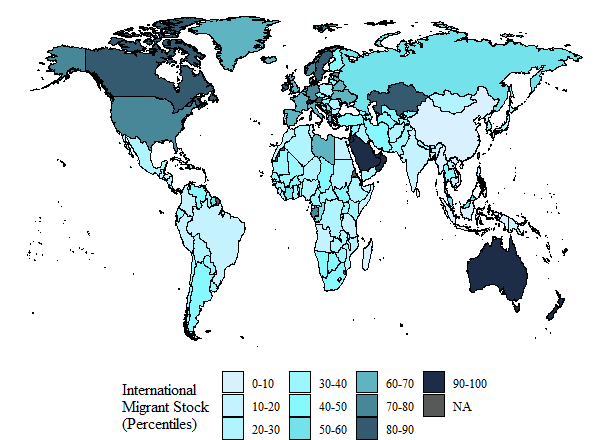
\includegraphics{../figures/maps/ims_map.png}
    \label{fig:1}
\textit{Note}: Data from the World Bank's International Migrant Stock (\% of total population), from the World Development Indicators. Elaborated by the Author. 
   \end{minipage}
   }
\end{figure}

The model in the fifth column of Table \ref{tab:1}, adds the Historical Index of Ethnic Fractionalization for 2013, which represents “the likelihood that two people chosen at random within a given country will be from different ethnic groups” \parencite[pp.1]{Drazanova.2019}. There is no data available for 2015 for this covariate, however, this two-year lag might help account for the fact that ethnic diversity takes time to accommodate. As reviewed before, a country that is more culturally diverse can be seen as more tolerant; migrants can feel more confident and hope to find people from a similar cultural background. The model results are consistent with this, and the other variables keep their significance with the exception of the ‘Raise’ policy dummy, which has a reduction in importance. This might happen because countries that desire to increase migration levels might also have relatively higher values of ethnic diversity, thus this variable better captures the effects of an open migration policy on migrant stocks. Unemployment presents unstable significance; I keep including it to see its relationship with new variables. 

The model in column 6 of Table \ref{tab:1} includes government expenditure. In this case, the policy dummies lose significance, and unemployment still has none. The policy dummies, unemployment and government expenditure are not jointly significant to this model. \textcite{Azad.2020} mentions that when a country is democratic, it tends to give migrants incentives to come, such as a good health system, safety, and security. Democracy may already include the information represented by government expenditure; thus, it is dropped in the following models along with the policy variables. This way I avoid losing sample size due to a lack of sufficient information for the territories in the World Bank and United Nations datasets. This is certainly a significant limitation to this empirical approach, since policy cannot be observed fully and may have an important effect on migrant stocks. Besides, the effect of democracy may be closely related to policy, since democratic countries might tend to establish restrictive migration policy. 

The effect of economic freedom proves to be important for the models, as significance is kept as well as its sign. Due to what is argued by \textcite{Holcombe.2015}, it is important to keep this covariate included in the model. They find that corruption is associated with the amount of regulation in the country; if this is so, I correct possible biases related to control of corruption when accounting for the days to start a business. Roughly, if more economic freedom implies less corruption, by leaving out the days required to start a business, an upward bias may arise on the control of corruption coefficient. This would overestimate the effect that higher government integrity has on migrant stocks. Including both these variables might also be important to estimate the effect of democracy more accurately, according to \textcite{Prada.2020}. 



\end{document}